\documentclass{sig-alternate}
\usepackage{multirow}
\usepackage{color}
\usepackage{colortbl}
\usepackage{picture}
\usepackage{algorithm}
\usepackage{algorithmicx}
\usepackage{algpseudocode}
\renewcommand{\algorithmicrequire}{\textbf{Input:}}
\renewcommand{\algorithmicensure}{\textbf{Output:}}
 

%timm tricks
\newcommand{\bi}{\begin{itemize}[leftmargin=0.4cm]}
\newcommand{\ei}{\end{itemize}}
\newcommand{\be}{\begin{enumerate}}
\newcommand{\ee}{\end{enumerate}}
\newcommand{\tion}[1]{\S\ref{sect:#1}}
\newcommand{\fig}[1]{Figure~\ref{fig:#1}}
\newcommand{\eq}[1]{Equation~\ref{eq:#1}}
 

\usepackage[shortlabels]{enumitem} 
\usepackage{times}
\newcommand{\subparagraph}{}
\usepackage{url}
\def\baselinestretch{1}


\setlist{nosep}
 \usepackage[font={small}]{caption, subfig}
\setlength{\abovecaptionskip}{1ex}
 \setlength{\belowcaptionskip}{1ex}

 \setlength{\floatsep}{1ex}
 \setlength{\textfloatsep}{1ex}
\usepackage[compact,small]{titlesec}
\DeclareMathSizes{7}{7}{7}{7} 
\pagenumbering{arabic}
\setlength{\columnsep}{7mm}

\begin{document}

\conferenceinfo{FSE}{'15 Bergamo, Italy}
\title{Phase Delay Increases  Repair Time. Not.}
\numberofauthors{3}
\author{
\alignauthor
Tim Menzies, \\Carter Pape\\
       \affaddr{CS, NcState, USA}\\
       tim.menzies@gmail.com,\\carterpape@gmail.com
\alignauthor
William Curtis,\\ Forrest Schull\\
\affaddr{SEI, CMU, USA}
wrn,fjshull@sei.cmu.edu
\alignauthor
Lucas \\Layman\\
       \affaddr{Fraunhofer Center,  USA}\\ 
       llayman@fc-md.umd.edu
} 


 
\maketitle
\begin{abstract}
This paper categorically rejects 
the myth that 
the longer a defect persists in a system, the harder
it is to remove that defect.  
This myth is very widely believed
and that the evidence for this myth dates back to certain
isolated studies dating from the 1970s. Recent evidence from
230 software projects from around the world shows that this
myth is completely false.

More important that our particular results, this paper
raises the methodological question of how a small number
of observations from the 1970s can become dogma for decades.
The obvious next question arising from this study is ``how
many other widely held beliefs in software engineering are
not supported by current data?''.
\end{abstract}

% A category with the (minimum) three required fields
\vspace{1mm}
\noindent
{\bf Categories/Subject Descriptors:} 
D.2.8 [Software Engineering]: Product metrics; 

 

\vspace{1mm}
\noindent
{\bf Keywords:} defect prediction, 

\section{Introduction}

\section{Related Work}

In their text Romabach laws

Kent Beck's original extreme programming text is big on this.

Historical  evidence for this dataes back to some studies in the 1970s. To the best of
our knowledge, not updated since. Regardless, as discussed in the next section, this

The first data on the cost to fix defects as a function of lifecycle phase date back to large systems in the late 70s from IBM~\cite{Fagan76}, TRW~\cite{Boehm76}, GTE~\cite{Daly77}, and Bell Labs~\cite{Stephenson76} (Figure~\ref{fig:cost-to-fix}). These studies suggest that the cost (in terms of effort) to find and fix an error monotonically increases with lifecycle phase. For large projects, the ratio of cost-to-fix in the requirements phase to cost-to-fix in operation is on the order of 1:100. Furthermore, cost function is superlinear, with the greatest rates of increase in the acceptance testing and operations phases.

\begin{figure}[!ht]
 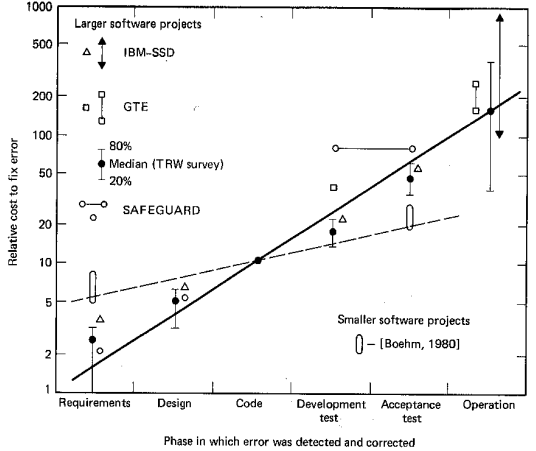
\includegraphics[width=3.3in]{boehm_cost-to-fix.png}
 \caption{Historical cost-to-fix curve. From~\cite{Boehm81}.}\label{fig:cost-to-fix}
 \end{figure}
 
In the 40 years since these initial studies, few studies have been published on the cost-to-fix curve as a function of lifecycle phase. Boehm~\cite{Boehm80} provides data suggesting that the cost-to-fix curve for small projects (from two student projects of 2000 deliverable source instructions) is flatter than for large projects (the dashed line of Figure~\ref{fig:cost-to-fix}). Shull et al.~\cite{Shull02} conducted a literature survey and held a series of e-workshops with industry experts on fighting defects. Workshop participants from Toshiba and IBM reported cost-to-fix ratios of 1:137 and 1:117 for large projects respectively~\cite{Shull02} -- the raw data points are not provided. One notable example to the traditional cost-to-fix curve is the CCPDS-R described by Royce~\cite{Royce98}: a million-line, safety-critical missile defense system (Figure~\ref{fig:royce}). In this project, design changes (including architecture changes) required approximately twice the effort of implementation and test changes, and the cost-to-fix in implementation and test phases increased slowly. Boehm~\cite{Boehm10} attributes this success to the CCPDS-R development process, which focused on removing architecture risk early in the development lifecycle.

\begin{figure}[!ht]
 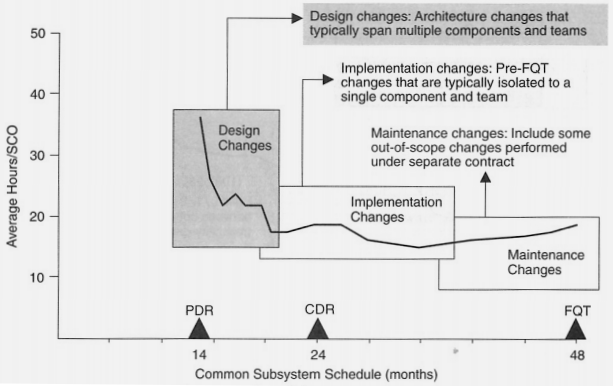
\includegraphics[width=3.3in]{Royce98.png}
 \caption{Exception to the rule - CCPDS-R case study cost-to-fix curve. From~\cite{Royce98}.}\label{fig:royce}
 \end{figure}
 
As discussed is \S\ref{sec:why-study}, one goal of agile methods is to flatten the cost-to-change curve~\cite{beck00}. Relatively little empirical data exists on this point. Clutterbuck et al.~\cite{Clutterbuck09} studied 5-month effort by a small-to-medium enterprise team developing a 71KLOEC web interface to a database application to implement 18 change requests (Figure~\ref{fig:clutterbuck}). Note that these were for new and changed user requirements, not defects. Clutterbuck et al. found the cost of change to be relatively flat until the later phases, with much of the effort spent in analysis of the change requests~\cite{Clutterbuck09}. Elssamadisy and Schalliol~\cite{Elssamadisy02} anecdotally report on the growing, high cost of rework in a 50 person, three-year, 500KLOEC Extreme Programming project as the project grew in size and complexity.

\begin{figure}[!ht]
 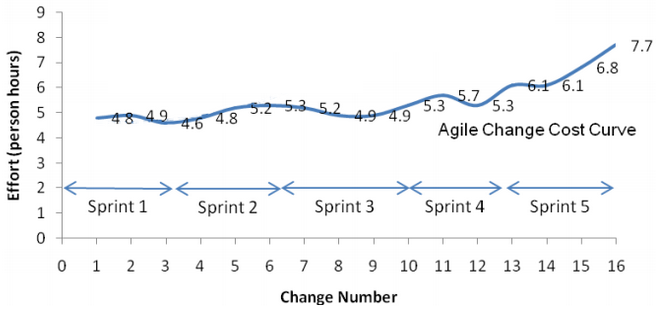
\includegraphics[width=3.3in]{clutterbuck.png}
 \caption{Cost of change from an agile case study. From~\cite{Clutterbuck09}.}\label{fig:clutterbuck}
 \end{figure}
 
 We note that previous work focuses on cost-to-fix as a function of lifecycle phase irrespective of when the defect was injected, that is, previous work analyzes the cost to fix a defect found in test regardless of whether that defect was a requirements error or a coding mistake. To our knowledge, our research represents the first large-scale study of phase delay.

\section{lucasSurvey}






Our survey collected data on software engineers' views of commonly held software engineering ``laws''.
One of the laws questioned relates directly to phase delay: ``Requirements errors are the most expensive to fix when found during production but the cheapest to fix early in development'' (from Glass~\cite{glass02} p.71 who references Boehm \& Basili~\cite{boehm01}). We abbreviate this law as RqtsErr. 

The survey was conducted in two phases using Amazon's Mechanical Turk. The first phase was conducted only with professional software engineers solicited through the Mechanical Turk\footnote{Professional software engineers were required to complete a pretest to verify their status as a professional or open source software developer and to confirm their knowledge of basic software engineering terminology and technology.}, and the second survey was conducted Program Committee members of the ESEC/FSE and ICSE conferences solicited via email.

The respondents answered the following questions for the laws they were presented: \newline
\textbf{Agreement:} ``Based on your experience, do you agree that the statement above is correct?'' A Likert scale captured the agreement score from Strongly Disagree to Strongly Agree. A text box was provided to explain the answer. \newline
\textbf{Applicability:} ``To the extent that you believe it, how widely do you think it applies among software development contexts?'' The possible answers were presented as a scale from -1 to 5:
\begin{itemize}
\item I don't know (-1)
\item This law does not apply at all (0)
\item Applies in a very narrow range of projects  (1)
\item Rarely applies (2)
\item Occasionally applies (3)
\item Very frequently applies (4)
\item Always applies (5)
\end{itemize}
Respondents were required to explain the applicability score in a text box.

Participants were presented with the RqtsErr law and others drawn from \cite{glass02} and \cite{endres03}. The PC member survey contained an additional question on ``In general, the longer errors are in the system (requirements errors, design errors, coding errors, etc.), the more expensive they are to fix'' (PhaseDelay for short). Responses were recorded using the Agreement question Likert scale. 

Summary statistics for the agreement and applicability scores for the RqtsErr and PhaseDelay laws are presented in Figure~\ref{fig:survey_results}. Responses whose Applicability response was ''I don't know'' are ommitted from analysis.


\begin{figure}[!ht] 
\scriptsize
\begin{center}
\subcaption{Practitioner survey}
\begin{tabular}{l|c|c|c|c|c}
Law & N & \multicolumn{2}{c}{agreement} & \multicolumn{2}{c}{applicability} \\ 
 & & $\bar{x}$ & $\tilde{x}$ & $\bar{x}$ & $\tilde{x}$ \\
\hline 
\textbf{Rqts errors are most expensive...} & 16 & 4.6 & 5 & 4.2 & 4 \\ 
Process maturity improves output & 17 & 4.4 & 4 & 3.9 & 4 \\ 
Most time is spent removing errors & 16 & 4.1 & 4 & 3.9 & 4 \\ 
Missing reqts are hardest to fix & 17 & 4.1 & 4 & 4.0 & 4 \\
Reuse increases prod. and qual. & 16 & 3.9 & 4 & 3.8 & 4 \\
OO-programming reduces errors & 13 & 3.9 & 4 & 3.5 & 4 \\
80-20 rule (defects to modules) & 12 & 3.8 & 4 & 4.0 & 4 \\
Adding manpower to a late project & 15 & 3.7 & 4 & 3.7 & 4 \\
Inspections can remove 90\% of defects & 18 & 3.3 & 4 & 3.5 & 4 \\
Smaller changes have higher error density & 14 & 2.8 & 3 & 3.4 & 3.5 \\
A developer is unsuited to test own code & 17 & 2.6 & 3 & 3.5 & 4
\end{tabular} 
\bigskip
\subcaption{Researcher survey}
\begin{tabular}{l|c|c|c|c|c}
Law & N & \multicolumn{2}{c}{agreement} & \multicolumn{2}{c}{applicability} \\ 
 & & $\bar{x}$ & $\tilde{x}$ & $\bar{x}$ & $\tilde{x}$ \\
\hline 
Process maturity improves output & 4 & 4.0 & 4 & 4.0 & 4 \\
\textbf{Rqts errors are most expensive...} & 30 & 3.8 & 4 & 3.8 & 4   \\ 
80-20 rule (defects to modules) & 6 & 3.7 & 4 & 3.5 & 4 \\
\textbf{PhaseDelay} & 30 & 3.6 & 4 & -- & --  \\ 
Missing reqts are hardest to fix & 7 & 3.6 & 4 & 3.7 & 4 \\
Adding manpower to a late project & 4 & 3.5 & 4 & 3.5 & 4 \\
Inspections can remove 90\% of defects & 7 & 3.4 & 4 & 3.6 & 3 \\
Reuse increases prod. and qual. & 6 & 3.3 & 4 & 3.0 & 4 \\
OO-programming reduces errors & 6 & 3.2 & 4 & 2.7 & 3 \\
Most time is spent removing errors & 6 & 2.8 & 3 & 3.2 & 4 \\ 
Smaller changes have higher error density & 4 & 2.8 & 3 & 4.0 & 4 \\
A developer is unsuited to test own code & 7 & 2.1 & 2 & 2.4 & 3
\end{tabular} 

\end{center}
\caption{Agreement and applicability of software engineering axioms.}
\label{fig:survey_results}
\end{figure}

While the practitioners strongly believed in the law, researchers were less firm. In the free response texts, most participants agreed that addressing errors late may mean system redesign unless the system and the affected requirement are simple/trivial. Further, any changes to the production system have additional complexity (compared to changes while system in development) due to users, data existence, and architecture dependencies. The researchers who disagreed with the law generally asserted that requirements change can be expensive, but that depends on the process used (e.g., agile vs. waterfall) and the adaptability of the system architecture.

Overall, the RqtsErr law was the most agreed upon and most applicable law of 11 surveyed amongst practitioners, and the second most agreed upon law amongst researchers. The survey results seem to confirm that the notion that phase delay escalates cost-to-fix is a widely-held belief in software engineering.

\section{billTSP}

\section{carterCharts}

anything

\section{Conclusion}

\section*{Acknowledgements}
This work was partially funded by an National Science
Foundation grant NSF-CISE 1302169.

\vspace*{0.5mm}
\scriptsize

\bibliographystyle{unsrt}
\bibliography{refs} 


\end{document}
